\documentclass{article}
\usepackage[utf8]{inputenc}
\usepackage{amsmath}
\usepackage{amsthm}
\usepackage{amssymb}
\usepackage{mathtools}
\usepackage{graphicx}
\usepackage{float}
\graphicspath{ {./images/} }

\title{Models of Computation Notes}
\author{William Guest}
\date{January 2023}

\newtheorem{thm}{Theorem}
\newtheorem{dummy}{Theorem}
\newtheorem{defn}[dummy]{Def}

\newcommand{\xto}[1]{ \overset{#1}{\to} }

\newcommand{\Enum}[2]{ #1_1, #1_2, \ldots, #1_#2 }
\newcommand{\Trans}[3]{ #1 \xrightarrow{ #2 }\mathrel{\vphantom{\to}} #3 }
\newcommand{\Translong}[3]{ #1 \xrightarrow{ #2 }\mathrel{\vphantom{\to}^*} #3 }
\newcommand{\dTrans}[3]{ #1 \xRightarrow{ #2 }\mathrel{\vphantom{\to}} #3 }
\newcommand{\dTranslong}[3]{ #1 \xRightarrow{ #2 }\mathrel{\vphantom{\to}^*} #3 }

\newcommand{\eqdef}[0]{ \overset{\text{def}}{=} }
\newcommand{\blank}[0]{\textvisiblespace}
\newcommand{\encode}[1]{\langle #1 \rangle}

\begin{document}

\maketitle

\section{Regular Languages}

    \subsection{Deterministic Finite Automata}

    \begin{defn}

        A \textbf{deterministic finite automata (DFA)}  is a 5-tuple $(Q, \Sigma, \delta, q_0, F)$ where
        \begin{itemize}
            \item $Q$ is a finite set called the states
            \item $\Sigma$ is a finite set called the alphabet
            \item $\delta : Q \times \Sigma \to Q$ is the transition function
            \item $q_0$ is the start state
            \item $F \subseteq Q$ is the set of accepting states
        \end{itemize}
    
    \end{defn}

    We write $\Trans{q}{a}{q'}$ to mean $\delta(q,a) = q'$. \\
    
    Let $M = (Q, \Sigma, \delta, q_0, F)$ be a DFA. For $w = a_1a_2 \ldots a_n$ a string over $\sigma$, we write $q \xto{w}* q'$ if there exists states $\Enum{q}{n} = q'$ such that
    \[ q \xto{a_1} q_1 \xto{a_2} \ldots \xto{a_n} q_n = q' \]
    Note that 
    \[ \Translong{q}{\epsilon}{q'} \text{ iff } q = q' \]

    and

    \[ \Translong{q}{a}{q'} \text{ iff } q \xto{a} q' \]

    $L(M)$, the language \textbf{recognised} by the DFA M, consists of all strings $w$ over $\Sigma$ satisfying $\Translong{q_o}{w}{q}$ where q is an accepting state. 

    \begin{defn}
        A language is called \textbf{regular} if some DFA recognises it. 
    \end{defn}

    \subsection{Non-Deterministic Finite Automata}

    \begin{defn}

        A nondeterministic finite automata (NFA) is a 5-tuple $(Q, \Sigma, \delta, q_0, F)$ where
        \begin{itemize}
            \item $Q$ is a finite set called the states
            \item $\Sigma$ is a finite set called the alphabet
            \item $\delta : Q \times (\Sigma \cap \{ \epsilon \}) \to \mathcal{P}(Q)$ is the transition function
            \item $q_0$ is the start state
            \item $F \subseteq Q$ is the set of accepting states
        \end{itemize}
    
    \end{defn}

    We write $\Trans{q}{a}{q'}$ to mean $\delta(q,a) = q'$. \\ \\

    Let $N = (Q, \Sigma, \delta, q_0, F)$ be an NFA. Let $\dTrans{q}{w}{q'}$ be defined by:
    \begin{itemize}
        \item $\dTrans{q}{\epsilon}{q'}$ iff $q = q'$ or there is a sequence $q \xto{\epsilon} \ldots \xto{\epsilon} q'$ of one or more $\epsilon$-transitions in $N$ from $q$ to $q'$.
        \item For $w = a_1\ldots a_{n+1}$ where each $a_i \in \sigma$, $\dTrans{q}{w}{q'}$ iff there are $q_1, q_1', \ldots, q_{n+1}, q_{n+1}'$ such that
        \[ \dTrans{q}{\epsilon}{q_1} \xto{a_1} \dTrans{q_1'}{\epsilon}{q_2} \xrightarrow{a_2} \ldots \dTrans{q_n'}{\epsilon}{q_{n+1}} \xto{a_{n+1}} \dTrans{q_{n+1}'}{\epsilon}{q'} \]
    \end{itemize}

    $L(N)$, the language recognised by N, consists of all strings $w$ over $\Sigma$ satisfying $\dTrans{q_0}{w}{q}$, where $q$ is an accepting state. 
    \begin{thm}
    Every NFA has an equivalent DFA. 
    \end{thm}
    This is proved by subset construction, each state in the DFA is a member of the powerset of states in the NFA. 

    If we fix an NFA $N = (Q_N, \Sigma_N, \delta_N, q_N, F_N)$, then we construct a DFA $\mathcal{P}(N) = (Q_{\mathcal{P}N}, \Sigma_{\mathcal{P}N}, \delta_{\mathcal{P}N}, q_{\mathcal{P}N}, F_{\mathcal{P}N})$ by
    \begin{itemize}
        \item $Q_{\mathcal{P}N} \eqdef \{ S \ | \ S \subseteq Q_N \}$
        \item $\Sigma_{\mathcal{P}N} \eqdef \Sigma_N$
        \item $\Trans{S}{a}{S'}$ in $\mathcal{P}N$ iff $S' = \{ q' \ | \ \exists q \in S.( \dTrans{q}{a}{q'} \text{ in } N) \}$
        \item $q_{\mathcal{P}N} \eqdef \{ q \ | \ \dTrans{q_N}{\epsilon}{q}\}$
        \item $F_{\mathcal{P}N)} \eqdef \{ S \in Q_{\mathcal{P}N} \ | \ F_N \cap S \neq \emptyset \} $
    \end{itemize}
    
    
    \subsection{Regular Operations}

    Let A and B be languages. Define 
    \begin{itemize}
        \item Union - $A \cup B = \{ x | x \in A \text{ or } x \in B \}$ 
        \item Concatenation - $A \cdot B = \{ xy \ | \ x \in A \text{ and } y \in B \}$ 
        \item Star - $A^* = \{ x_1 x_2 \ldots x^k \ |  \ k \geq 0 \text{ and each } x_i in A \}   $
    \end{itemize}

    \begin{thm}
        Regular languages are closed under union, concatenation and star. (If $A_1$ and $A_2$ are regular languages, then so are $A_1 \cup A_2$, $A_1 \cdot A_2$, and $A_1^*$)
    \end{thm}

    Take NFAs $N_1$ and $N_2$ that recognise $L(N_1)$ and $L(N_2)$ respectively.  \\

    We can see that regular languages are closed under union by constructing a new NFA from $N_1$ and $N_2$ which adds a new start state outside of each NFA, and joins them to each start state of $N_1$ and $N_2$ via $\epsilon$-transitions. 
    
    \begin{figure}[h!]
        \centering
        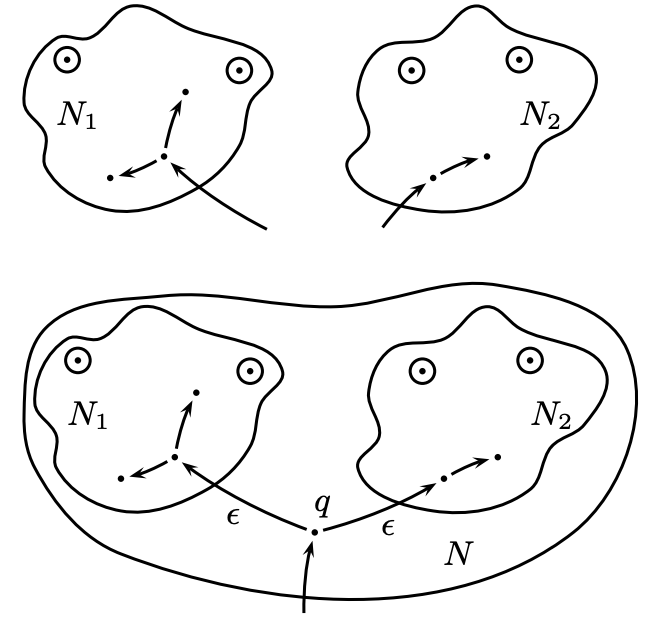
\includegraphics[scale=0.5]{images/union.png}
        \caption{Union Construction}
        \label{fig:union}
    \end{figure}

    To show that regular languages are closed under concatenation, we connect each accepting state of $N_1$ to the start state of $N_2$ via $\epsilon$-transitions. The start state of the new NFA is the start state of $N_1$, the accepting states are the accepting states of $N_2$. 

    \begin{figure}[H]
        \centering
        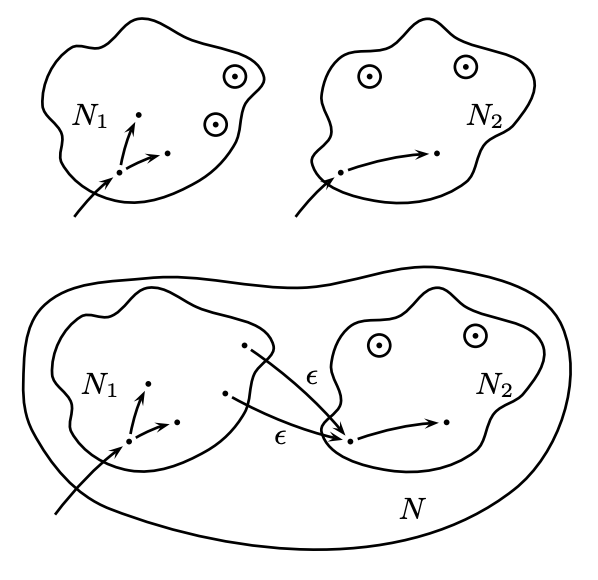
\includegraphics[scale=0.5]{images/concatenation.png}
        \caption{Concatenation Construction}
        \label{fig:concatenation}
    \end{figure}

    To show that regular languages are closed under star, we add a dummy accept state at the start which connects via an $\epsilon$-transition to the start state of $N_1$. We also connect each accept state to the start state of $N_1$ via $\epsilon$-transitions. Note that we can't just make the start state of $N_1$ an accept state as this would not account for cases where the start state can be reached via transitions that aren't $\epsilon$-transitions from the accept states in $N_1$

    \begin{figure}[H]
        \centering
        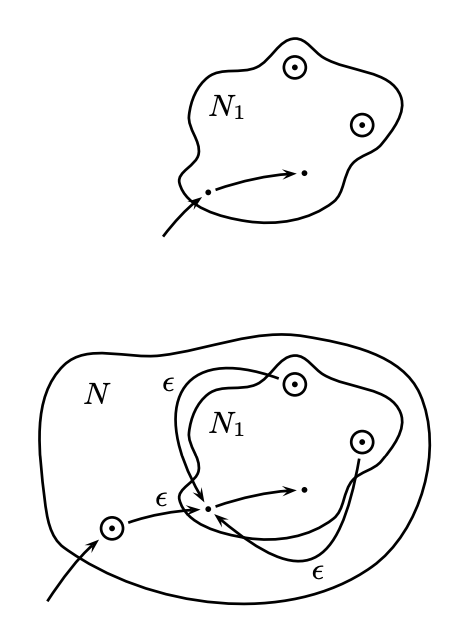
\includegraphics[scale=0.5]{images/star.png}
        \caption{Star Construction}
        \label{fig:star}
    \end{figure}

    \subsection{Regular Expressions}

    \begin{defn}
        We fix an alphabet $\Sigma$. We define regular expression $E$ and the language denoted by $E$, $L(E)$ recursively:
        \begin{itemize}
            \item The constants $\epsilon$ and $\emptyset$ are regular expressions, with $L(\epsilon) \eqdef \{ \epsilon\}$ and $L(\emptyset) \eqdef \{ \emptyset\}$.
            \item For $a \in \Sigma$, $a$ is a regular expression, with $L(a) \eqdef \{ a \}$.
            \item If $E$ and $F$ are regular expressions, then so are $(E+F)$, $(E \cdot F)$, $(E^*)$ with 
            \begin{align*}
                L((E+F)) &\eqdef L(E) \cup L(F) \tag*{Union} \\
                L((E \cdot F)) &\eqdef L(E) \cdot L(F) \tag*{Concatenation} \\
                L((E^*)) &\eqdef (L(E))^* \tag*{Star} \\
            \end{align*}
        \end{itemize}

        Note $+$ is sometimes written as $\cup$ or $|$, and $(E \cdot F)$ is sometimes written as $(EF)$. Note also that the order of precedence is star, concatenation, union, so $(0 + 1)01^*)$ is formally $((((0+1) \cdot 0) \cdot (1^*)) \cdot 0 )$.
        
    \end{defn}

    We have some equivalences for regular expressions:
    \begin{align*}
        (E + F) + G &\equiv E + (F + G) \tag*{Associativity} \\
        (EF)G &\equiv E(FG) \tag*{Associativity} \\
        E+F &\equiv F+E \tag*{Commutativity} \\ 
        E \emptyset &\equiv \emptyset \\ 
        \emptyset^* &\equiv \epsilon \\
        E + \emptyset \equiv E &\equiv \emptyset + E\\
        E \epsilon \equiv E &\equiv \epsilon E\\
    \end{align*}
    
    \begin{thm}[Kleene's Theorem]
        Let $L \subseteq \Sigma$. The following are equivalent:
        \begin{itemize}
            \item $L$ is regular
            \item $L$ is denoted by some regular expression E, i.e. $L = L(E)$
        \end{itemize}
    \end{thm}

    Proving that any regular expression has an NFA is simple, there are NFAs that recognise $\epsilon$, $\emptyset$ and $a$, for all $a \in \Sigma$. Since languages are closed under union, concatenation and star, for regular expressions $E$ and $F$, with NFAs $N_E$ and $N_F$ respectively, there are also NFAs that recognise $L(N_E) \cup L(N_F), L(N_E) \cdot L(N_F)$, and $(L(N_E))^*$, which are equivalent to $E + F$, $E \cdot F$, $E^*$ respectively. \\  

    To prove that a given NFA has a regular expression, we construct a regular expression recursively. Given NFA $M = (Q, \Sigma, \delta, q, F)$, for $X \subseteq Q$ and $q, q' \in Q$, we construct on induction on the size of $X$, the regular expression
    \[ E^X_{q,q'} \]
    which denotes the set of strings such that there is a path from $q$ to $q'$ labelled $w$, i.e. $\dTrans{q}{w}{q'}$ such that all \textbf{intermediate} states along that path lie in X. Hence to find the regular expression for $M$ is
    \[ L(M) = \sum_{f \in F} E^Q_{q_0,f}\]
    To construct such a regular expression, we construct recursively on the size of $X$ The base case is when $X = \emptyset$. For $q = q'$, take
    \[ E^\emptyset_{q,q'} \eqdef 
        \begin{cases}
    			a_1 + \ldots + a_k & \text{if $k \geq 0$}\\
                \emptyset & \text{otherwise}
        \end{cases}\]
    and for $q=q'$, take
    \[ E^\emptyset_{q,q'} \eqdef 
        \begin{cases}
    			a_1 + \ldots + a_k + \epsilon & \text{if $k \geq 0$}\\
                \epsilon, & \text{otherwise}
        \end{cases}\]
        In this way, we only can go from one state to another if there is a direct transition, or if the state we are on currently is the state that we are trying to get to, as there are no intermediate states. \\ \\
        For the inductive step, we choose some $r \in X$ called the \textit{separating state}. Any path from $q$ to $q'$ must either:
        \begin{itemize}
            \item Never visit $r$
            \item Visit $r$, loop from $r$ to $r$ some non-negative number of times, and then visit $p'$
        \end{itemize}
        Hence for non-empty $X$, we take
        \[ E^X_{q,q'} \eqdef E^{X - \{r\}}_{q,q'} + E^{X - \{r\}}_{q,r} \cdot (E^{X - \{r\}}_{r,r})^* \cdot E^{X - \{r\}}_{r,q'} \]
        To simplify this process, we choose a separating state that splits the automaton as much as possible. 
    \subsection{Kozen's Axioms}
        Kozen's axioms define a set of rules and equivalences that define equivalences between regular expressions. The axioms are sound (meaning that all rules are valid) and complete (meaning that any equivalence between regular expression can be derived from these axioms). 
        \begin{enumerate}
            \item $E + (F + G) \equiv (E + F) + G$
            \item $E + F \equiv F + E$
            \item $E + \emptyset \equiv E$
            \item $E + E \equiv E$
            \item $(EF)G \equiv E(FG) $
            \item $\epsilon E \equiv E \epsilon \equiv E$
            \item $E(F + G) \equiv EF + EG$
            \item $(E + F)G \equiv EG + FG$
            \item $\emptyset E \equiv E \emptyset \equiv \emptyset$
            \item $\epsilon + EE^* \equiv E^*$
            \item $\epsilon + E^* E \equiv E^*$
            \item $F + EG \leq G \implies E^*F \leq G$
            \item $F + GE \leq G \implies FE^* \leq G$
        \end{enumerate}
        where $E \leq F$ means $E + F \equiv F$, which is true iff $L(E) \subseteq L(F)$.
    \subsection{Characterisations of Regular Languages}
        \subsubsection{The Pumping Lemma}
        The pumping lemma is a way of proving that languages are not regular. It is \textit{not} a way of proving that languages are regular. 
        \begin{thm}
            If $A$ is a regular language, then there is some number $p$, the pumping length,  such that if $s \in A$ is of length at least $p$, then we can divide $s$ into three pieces $s = xyz$ such that
            \begin{itemize}
                \item for each $i \geq 0$, $xy^iz \in A$
                \item $|y| > 0$
                \item $|xy| \leq p$
            \end{itemize}
        \end{thm}
        Intuitively, this is the case because a regular language corresponds to an NFA with a finite number of states, so taking the pumping length to be the number of states, we must see that any word accepted by a regular language longer than $p$, must loop. \\ \\
        In practice we assume that a language is regular, choose some word in the language for an arbitrary pumping length and use this to derive a word that is not in the language, which is a contradiction. 
        \begin{thm}
            If for all $p \geq 1$ there exists some $s \in L$ with $|s| \geq p$ such that for all $x, y, z \in \Sigma^*$ with $s = xyz$ and $|xy| \leq p$ there is an $i \geq 0$ such that $xy^iz \notin L$, then $L$ is not regular. 
        \end{thm}
        \subsection{Myhill-Nerode Theorem}
        The Myhill-Nerode theorem provides an exact characterisation of regular languages, we can use it to determine when a language is regular or not. \\ \\
        We first define an equivalence relation. Let $x, y \in \Sigma^*$ be strings and let $L \in \Sigma^*$. We say that $x$ and $y$ are L-indistinguishable ($x \equiv_L y$) if for every $z \in \Sigma^*$,
        \[ xz \in L \text{ iff } yz \in L\]
        We define the index of a regular language to be the number of equivalence classes of $\equiv_L$. 
        \begin{thm}[Myhill-Nerode Theorem]
            A language is regular iff $\equiv_L$ has finite index. Moreover, the index is the number of states of the \textit{smallest} DFA that recognises $L$. 
        \end{thm}
        This comes from the fact that if $L$ is recognised by a DFA with $k$ states then there are at most $k$ equivalence classes, and that if $L$ has a finite index $k$, then there it is recognised by a DFA with $k$ states. 
\section{Context-Free Languages}
    \subsection{Context-Free Grammars}
    \begin{defn}
        A \textbf{Context-Free Grammar (CFG)} is a 4-tuple $G = (V,\Sigma,\mathcal{R},S)$ where
        \begin{itemize}
            \item $V$ is a finite set of \textbf{variables}
            \item $\Sigma$ is finite set of \textbf{terminals} (disjoint from $V$)
            \item $\mathcal{R}$ is a finite set of \textbf{rules} or productions. 
            \begin{itemize}
                \item A rule is an element of $V \times (V \cup \Sigma)^*$, written $A \to w$
                \item We write $A \to \alpha \ | \ \beta \ | \ \gamma$ to mean $A \to \alpha$, $A \to \beta$, $A \to \gamma$
            \end{itemize}
            \item $S \in V$ is the start symbol. 
        \end{itemize}
    \end{defn}
    Given a CFG $G$, we can define a binary relation, $\Rightarrow$ over $(V \cup \Sigma)^*$ as
    \[ uAv \Rightarrow uwv \]
    for each $u,v \in (V \cup \Sigma)^*$, for each $A \to w$ in $\mathcal{R}$. \\ \\
    We define $\Rightarrow^*$ as the reflexive and transitive closure of $\Rightarrow$. Hence a language generated by some CFG $G$ can be written as 
    \[ L(G) = \{ w \in \Sigma^* \ | \ S  \Rightarrow^* w\} \]
    A CFG is right-linear if every rule is of the form $A \to wT$ or $A \to w$, where $R,T$ are variables and $w$ is a terminal. 
    \begin{thm}
        A language is regular iff it is generated by a right-linear CFG. 
    \end{thm}
    We prove this by showing that all right-linear CFGs are equivalent to a \textit{strongly right-linear} CFG, meaning all rules are of the form $A \to T$, $A \to wT$ or $A \to \epsilon$, and that each strongly right-linear CFG is equivalent to a DFA/NFA. 
    \subsection{Parse Trees}
    A CFG derivation can determine a parse tree. Given a CFG $G = (V,\Sigma,\mathcal{R},S)$, a parse tree is a tree satisfying
    \begin{itemize}
        \item The root of the the tree is $S$
        \item Each vertex of the parse tree is a variable, a terminal or $\epsilon$
        \item If $A \to B_1, \ldots, B_k$ is a rule, then $B_1, \ldots, B_k$ are the children of A
        \item Leaf nodes are variables and interior nodes are terminals
    \end{itemize}
    \begin{figure}[h]
        \centering
        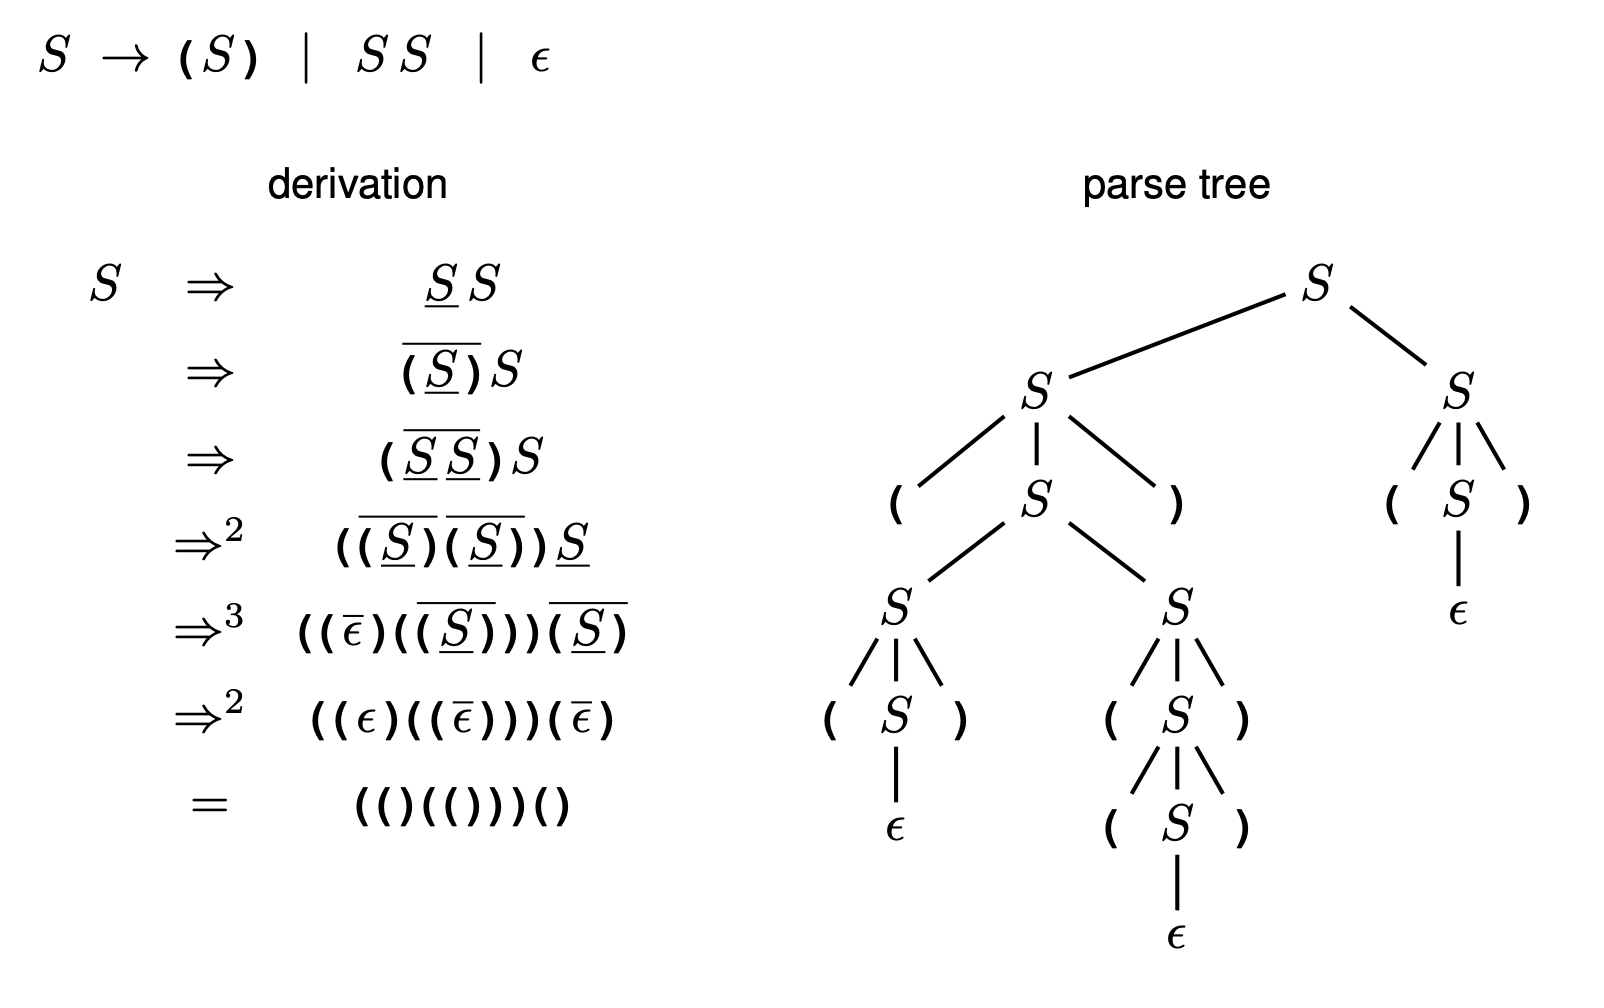
\includegraphics[scale=0.5]{images/parsetree.png}
        \caption{A CFG derivation and a parse tree}
        \label{fig:parsetree}
    \end{figure}
    \subsection{Ambiguity}
    Two derivations are \textit{essentially different} if they determine different parse trees. In some CFGs, a string may have different derivations, in these cases the CFG is \textbf{ambiguous}. A \textbf{leftmost derivation} is a derivation in which the leftmost variable is chosen for replacement. A CFG $G$ is ambiguous if there is some word in the language of $G$ that has two or more different leftmost derivations. Languages are \textbf{inherently ambiguous} if they can only be generated by ambiguous grammars. 
    \subsection{Pumping Lemma}
        \begin{thm}
            If $L$ is a context-free language, then there is a number $p$, the \textbf{pumping length} such that if $w \in L$ is of length at least $p$, then $w$ can be divided into five pieces $w = uxyzv$ such that
            \begin{itemize}
                \item For each $i \geq 0$, $ux^iyz^iv \in L$
                \item $|xz| > 0$
                \item $|xyz| \leq p$
            \end{itemize}
        \end{thm}
    \subsection{Chomsky Normal Form}
        A CFG is in Chomsky Normal Form if every rule is of the form $A \to BC \ | \ a$, where $a$ is any terminal and $A,B,C$ are variables with $B$ and $C$ not the start variable. We also permit $S \to \epsilon$
        \begin{thm}
            Any CFL can be generated by a CFG in Chomsky Normal Form
        \end{thm}
    \subsection{Non-Deterministic Pushdown Automata}
        Just as how regular languages are recognised by DFAs and NFAs, context-free langugages are recognised by NDPAs. 
        \begin{defn}
            A \textbf{Non-Deterministic Pushdown Automata (NDPA)} is a 7-tuple $(Q,\Sigma, \Gamma, \delta, q_0, \bot, F)$ such that $Q,\Sigma, \Gamma, \delta, F$ are all finite sets and
            \begin{itemize}
                \item $Q$ is the set of states
                \item $\Sigma$ is the input alphabet
                \item $\Gamma$ is the stack alphabet
                \item $\delta : Q \times (\Sigma \cup \{ \epsilon \}) \times \Gamma \to \mathcal{P}(Q \times \Gamma^*)$ is a transition function
                \item $q_0 \in Q$ is the start state
                \item $\bot \in \Gamma$ is the inital start symbol
                \item $F \subseteq Q$ is the set of accept states
            \end{itemize}
        \end{defn}
        A NPDA $M$ has \textit{configurations} describing the current state of the NPDA, the portion of the input yet unread and the current stack contents. The start configuration is
        \[ (q_0, w, \bot) \]
        meaning that $M$ always starts in the start state with its input head scanning the leftmost input symbol and the stack containing $\bot$. \\ \\
        We can then define a next-configuration relation that describes how $M$ moves from one configuration to another in one step. 
        \begin{itemize}
            \item If $(q, \gamma) \in \delta(p, a, A)$ then for any $v \in \Sigma^*$ and $\beta \in \Gamma^*$,
            \[ (p, av, A\beta) \to (q,v,\gamma \beta) \]
            (We consume the input symbol $a$, we pop $A$ and replace it with $\beta$)
            \item If $(q, \gamma) \in \delta(p, \epsilon, A)$ then for any $v \in \Sigma^*$ and $\beta \in \Gamma^*$,
            \[ (p, v, A\beta) \to (q,v,\gamma \beta) \]
            (We don't consume any input)
        \end{itemize}
        Similarly to DFAs and NFAs, we can define the reflexive, transitive closure of $\to$,
        \[ \Trans{C}{0}{D} \iff C=D \]
        \[ \Trans{C}{n+1}{D} \iff \exists E s.t. \Trans{C}{n}{E} \land E \to D\]
        and define $\Trans{C}{*}{D}$ just when there is some $n \geq 0$ such that $\Trans{C}{n}{D}$. \\ \\
        We say that $M$ \textbf{accepts an input x by final state} if there is some $q \in F$ and some $\gamma \in \Gamma^*$ such that $\Trans{(q_0, x, \bot)}{*}{(q, \epsilon, \gamma)}$. The \textbf{language} of $M$, $L(M)$ is the set of strings accepted by $M$. We also have another accepting convention, $M$ \textbf{accepts an input x by empty stack} if for some $q \in Q$, $\Trans{(q)}{\epsilon}{\epsilon}$, hence meaning the set $F$ is irrelevant. The two conventions are equivalent. 
        \begin{thm}
            A language is context free iff there is some NPDA that recognises it.
        \end{thm}
        We can show that any given CFG has an NDPA that simulates it. Given $G$, we can construct $P_G$ by
        \begin{enumerate}
            \item Place the start variable on the stack.
            \item Repeat forever: Pop top-of-stack $x$, there are three cases:
            \begin{enumerate}
                \item $x$ is a variable $A$. Nondeterministically choose a rule for $A$ and replace $A$ by the rule's rhs. 
                \item $x$ is a terminal $a$. Read the next input symbol and compare it with $a$. If they do not match, then reject this branch. 
                \item $x = \bot$ We enter the accept state. 
            \end{enumerate}
        \end{enumerate}
        To show that any given NPDA has an equivalent CFG, we first show that any NPDA has an equivalent NPDA with one state. Given an NPDA $M=(Q, \Sigma, \Gamma, \delta, s, \bot, \{t\}$ we constuct an NPDA $M'=({ * }, \Sigma, \Gamma', \delta', *,  \langle s \ \bot \ t\rangle, \bot, \emptyset$, where
        \[ \Gamma' = Q \times \Gamma \times Q \]
        and for each transition 
        \[ (q_0, B_1, \ldots, B_k) \in \delta(p, c, A) \]
        where $c \in \Sigma \cup \{ \epsilon \}$, we include in $\delta'$,
        \[ *, \langle q_0 \ B_1 \ q_1 \rangle \langle q_1 \ B_2 \ q_2 \rangle \ldots \langle q_{k-1} \ B_k \ q_k \rangle ) \in \delta'(*, c, \langle p \ A \ q_k)  \]
        for all choices of $q_1, \ldots, q_k$. Intitively, $M'$ simulates $M$ guessing non-deterministically what state $M$ will be in at certain points in the future, saving those guesses on the stack, and verifying later that those guesses were correct. \\ \\
    
        Hence given an NPDA $M$ with only one state, $( \{ q \}, \Sigma, \Gamma, \delta, q, \bot, \emptyset )$ that accepts by empty stack, we define a CFG $G_M = (\Gamma, \Sigma, P, \bot)$ where $P$ contains a rule 
        \[ A \to cB_1 \ldots B_k \]
        for every transition,$(q, B_1 \ldots B_k) \in \delta(q, c, A)$ where $c \in \Sigma \cup \{  \epsilon \}$. Hence $L(M) = L(G_M)$. 
    \subsection{Regular Operations}
        \begin{thm}
            Context free languages are closed under union, concatenation and star. 
        \end{thm}
        We can show this, given $G_1 = (\Gamma_1, \Sigma, \mathcal{R}_1, S_1)$ and $G_2 = (\Gamma_2, \Sigma, \mathcal{R}_2, S_2)$ with $\Gamma_1 \cap \Gamma_2 = \emptyset$, we can define the CFGs using the new start variable:
        \begin{align*}
            G_{\text{union}} &= (\Gamma_1 \cup \Gamma_2 \cup \{ S \}, \Sigma, \mathcal{R}_1 \cup \mathcal{R}_2 \cup \{ S \to S_1, S \to S_2 \}, S) \\ 
            G_{\text{concat}} &= (\Gamma_1 \cup \Gamma_2 \cup \{ S \}, \Sigma, \mathcal{R}_1 \cup \mathcal{R}_2 \cup \{ S \to S_1 S_2 \}, S) \\
            G_{\text{star}} &= (\Gamma_1 \cup \Gamma_2 \cup \{ S \}, \Sigma, \mathcal{R}_1 \cup \mathcal{R}_2 \cup \{ S \to S_1 S, S \to \epsilon \}, S) \\
        \end{align*}
        Then $L(G_{\text{union}}) = L(G_1) \cup  L(G_2)$, $L(G_{\text{concat}}) = L(G_1) \cdot L(G_2)$, and $L(G_{\text{star}}) = L(G)^*$ \\ \\
        Context-free languages are \textbf{not} closed under intersection. 
\section{Recursively Enumerable Languages}
    \subsection{Turing Machines}
    \begin{defn}
        A Turing Machine is a 9-tuple
        \[ (Q, \Sigma, \Gamma, \vdash, \blank, \delta, q_0, q_{acc}, q_{rej}) \]
        where
        \begin{itemize}
            \item $Q$ is a finite set (the states)
            \item $\Sigma$ is a finite set (the input alphabet)
            \item $\Gamma$ is a finite set (the tape alphabet)
            \item $\vdash \in \Gamma - \Sigma$ is the left endmarker
            \item $\blank \in \Gamma - \Sigma$ is the blank symbol
            \item $\delta \ : \ Q \times \Gamma \to Q \times \Gamma \times \{L, R \}$ is the transition function
            \item $q_0, q_{acc}, q_{rej}$ are the start, accept and reject states respectively. 
        \end{itemize}

        
    \end{defn}
    \begin{figure}[H]
        \centering
        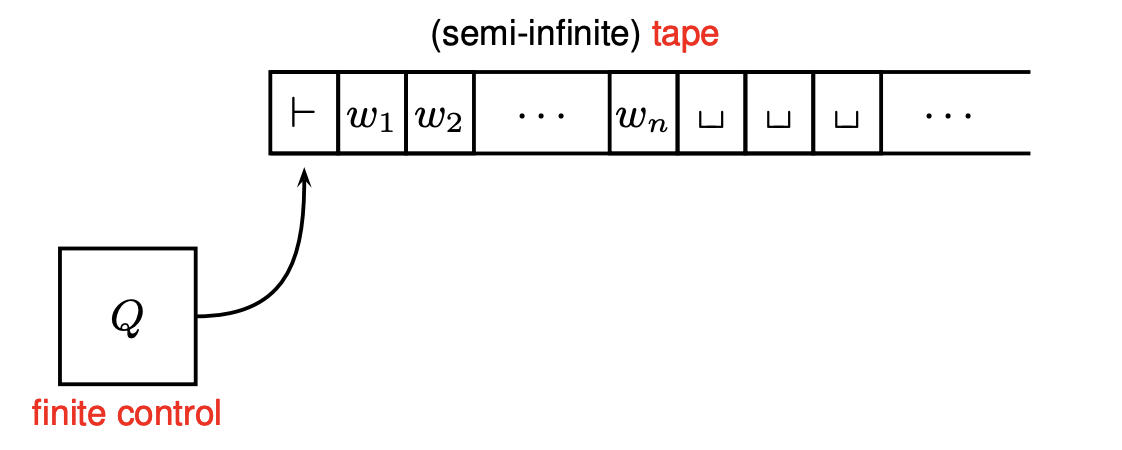
\includegraphics[scale=0.5]{images/turingmachine.png}
        \caption{Turing Machine}
        \label{fig:turingmachine}
    \end{figure}
    At the start of the computation, the contents of the Turing Machine are 
    \[ \vdash w_1, \ldots, w_n, \blank, \blank, \ldots \]
    where $w = w_1 \ldots w_n$ is the input string and the tape head is over $\vdash$, the left endmarker. To the right of the input word is an infinite number of $\blank$. 
    \begin{defn}
        A \textbf{configuration} of a Turing Machine is a triple $(u, q, v)$ where the current state is $q$, the current tape content is $u, v$ and the current head location is over the first symbol of $v$. 
    \end{defn}
    Hence we can define the next configuration relation $\to$ as 
    \begin{itemize}
        \item $(ua, q, bv) \to (u, q', acv)$ if $\delta(q, b) = (q',c,L)$
        \item $(ua, q, bv) \to (uac, q', v)$ if $\delta(q, b) = (q',c, R)$
    \end{itemize}
    We also define the transitive, reflexive closure of this relation $\Trans{}{*}{}$ as
    \begin{itemize}
        \item $\Trans{C}{0}{C} $ for all configurations $C$
        \item $\Trans{C}{n+1}{C''}$ iff $\Trans{C}{n}{C'}$ and $C' \to C''$
    \end{itemize}
    where $\Trans{C}{*}{C'}$ means there is some $n \geq 0$ such that $\Trans{C}{n}{C'}$.. \\ \\
    Intuitively, $\delta(q, a) = (q', b, L)$ means that when in state $q$, scanning symbol $a$, then enter state $q'$, write $b$ over the tape cell and move the head left by one cell. Note that the left endmarker is never overwritten and once the machine enters $q_{acc}$ or $q_{rej}$, it will never leave these states. \\ \\
    \begin{itemize}
        \item The \textbf{start configuration} of a Turing Machine on an input $w$ is $(\epsilon, q_0, \vdash w)$.
        \item An \textbf{accepting configuration}is any configuration with state $q_{acc}$
        \item A \textbf{rejecting configuration} is any configuration with state $q_{rej}$. 
        \item M \textbf{accepts} input $w$ just when $\dTrans{(\epsilon, q_0, \vdash w)}{*}{C}$
    \end{itemize}
    \subsubsection{Halting}
        When a TM $M$ starts on an input it may either \textbf{accept}, \textbf{reject}, or \textbf{loop forever}. We say that $M$ halts on an input if it either accepts it or rejects it. $M$ is \textbf{total} or a decider if it halts on all possible inputs. We call a language decidable if it is recognised by some total TM, in which case this TM decides the language. \\ \\
        A \textbf{recursively enumerable} language is a language such that there is a TM that halts and accepts when presented with any string in that language, \textit{although it may fail to halt when presented with a string not in that language}. A language $L$ is \textbf{co-RE} if its complement, $\overline{L}$ is recursively enumerable. \\ \\
        A language is decidable iff it is both RE and co-RE. If we have languages $L$ and $\overline{L}$ that are both RE, then we can simulate their corresponding TMs, accepting or rejecting when either one accepts or rejects. Since both $L$ and $\overline{L}$ are RE, this machine can never halt, so it must be a decider.\\ \\
        We can encode Turing Machines as strings over an alphabet. We write the encoding of the TM $M$ as $\encode{M}$.
    \subsection{Turing Machine Variations}
    \subsubsection{Multi-Tape Turing Machines}
    $k-tape$ TMs have $k$ semi-infinite tapes each with its own independent read/write head. Initially the input is occupied by the first tape, with the other tapes blank. In each step, the machine reads each of the $k$ symbols under its tape head and moves each tape head accordingly (different tape heads may move in different directions). The transition function is hence of the type
    \[ \delta \ : \ Q \times \Gamma^k \to Q \times \Gamma^k \times \{L, R\}^k \]
    Each multi-tape TM is equivalent to a single tape one. This is done by simulating each cell of the different tracks in one cell, using a marker in each subcell to track where the corresponding tape head is for the simulated track. Hence one move of the multi-tape TM is simulated by several moves of the single-tape TM, as the TM needs to traverse the tape, modifying the cells accordingly until it has modified all of the markers, at which point it returns to the left of the tape. 
    \subsubsection{Non-Deterministic Turing Machines}
    A NDTM is non-deterministic, so that at any point in the computation, it may proceed in several possible directions. If any of these directions accepts the input, then the entire NDTM accepts. 
    \begin{thm}
        A language is recognised by some TM iff it is recognised by some NDTM
    \end{thm}
    \subsubsection{Universal Turing Machines}
    A \textbf{universal TM} is a TM $U$ that can simulate the actions of any TM. For any TM $M$ and input $x$, $U$ accepts, rejects or loops $\encode{M,x}$ iff $M$ accepts, rejects or loops on $x$ respectively.\\ \\
    The universal TM has three tracks:
    \begin{itemize}
        \item The top track holds the transition function $\delta_M$ of the input TM $M$.
        \item The middle track holds the simulated contents of $M$'s tape
        \item The bottom track holds the current state of $M$, alongside the position of $M$'s tape head. 
    \end{itemize}
    Note that the input alphabet of $U$ and $M$ may be different. 
    \section{Decidability}
    Recall a language is decidable iff it is recognised by some total TM. \\ \\
    There are several decidable problems:
    \begin{itemize}
        \item DFA Acceptance
            \begin{itemize}
                \item Given a DFA $B$ and an input $w$, does $B$ accept $w$?
                \item $A_{DFA} = \{ \encode{B,w} \ | \ B \text{ is a DFA that accepts input sting $w$} \}$
                \item Construct a TM that on input $\encode{B,w}$ simulates $B$ on input $w$, accepting and rejecting if $B$ accepts or rejects $w$
            \end{itemize}
        \item DFA Emptiness
            \begin{itemize}
                \item Given a DFA $A$, is $L(A) = \emptyset$?
                \item $E_{DFA} = \{ \encode{A} \ | \ B \text{ is a DFA such that $L(A) = \emptyset$} \}$
                \item Construct a TM that on input $\encode{A}$ marks the start state of $A$, and repeatedly marks any state that has a transition coming into it from any marked state
                \item If no accept state is marked, \textit{accept}, otherwise \textit{reject}
            \end{itemize}
        \item DFA Equivalence
            \begin{itemize}
                \item Given two DFA's are they equivalent?
                \item $EQ_{DFA} = \{ \encode{A, B} \ | \ \text{$A$ and $B$ are DFAs such that $L(A) = L(B)$} \}$
                \item We use the idea that $P \subseteq Q$ iff $P \cap \overline{Q} = \emptyset$, using $T$ the algorithm for $E_{DFA}$
                \item On input $\encode{A,B}$, where $A,B$ are DFAs, run $T$ on $\encode{ (A \cap \overline{B}) \cup (\overline{A} \cap B) }$, accepting just when $T$ accepts. 
            \end{itemize}
        \item CFG Acceptance
            \begin{itemize}
                \item Given a CFG $G$ and an string $w$, can $G$ generate $w$?
                \item $A_{CFG} = \{ \encode{G, w} \ | \ \text{$G$ is a CFG that generates $w$} \}$ 
                \item We convert $G$ into Chomsky normal form, hence any derivation of $w$ has $2n - 1$ steps where $n = |w|$. 
                \item We then construct a TM that on input $\encode{G, w}$, converts $G$ into CNF, lists all derivations of length $2n - 1$ and accepts just when any of these derivations are $w$
            \end{itemize}
        \item CFG Emptiness
            \begin{itemize}
                \item Given a CFG $G$ is $L(G) = \emptyset$
                \item $E_{CFG} = \{ \encode{G} \ | \ \text{$G$ is a FG such that $L(G) = \emptyset$} \}$
                \item We construct a TM $T$, that on input $\encode{G}$, where $G = (V, \Sigma, R, S)$, marks all terminal symbols in $G$ and repeatedly marks any variables $A$, where $G$ contains a rule $A \to U_1 \ldots U_k$, where each $U_i \in \Sigma \cup V$ has been marked already.
                \item If the start symbol is not marked, \textit{accept}, otherwise \textit{reject}. 
            \end{itemize}
    \end{itemize}

    Note the problem of CFG equivalence is undecidable, we cannot use the techniques used in DFA equivalence as CFGs are not closed under intersection nor complementation. \\ \\
    The acceptance problem for TMs is recursively enumerable. 
    \[ A_{TM} = \{ \encode{M, w}, \text{$M$ is a TM that accepts input $w$} \} \]
    We can show that this is true by defining a TM $U$ that accepts $A_{TM}$: One input $\encode{M, w}$ where $M$ is a TM and $w$ is a string, 
    \begin{enumerate}
        \item Simulate $M$ on input $w$
        \item If $M$ ever enters its accept state, \textit{accept}: if $M$ ever enters its reject state, \textit{reject}. 
    \end{enumerate}
    Note that $U$ loops whenever $M$ loops, so $U$ is not a decider. \\ \\
    We can further see that $A_{TM}$ is undecidable, meaning that there is no decider for $A_{TM}$. We can prove this by contradiction, suppose there was a decider for $A_{TM}$, $H$. This means that
    \[ H(\encode{M,w}) = 
    \begin{cases}
        \textit{accept} & \text{if $M$ accepts $w$}\\
        \textit{reject} & \text{if $M$ does not accept $w$}
    \end{cases}
    \]
    We can then construct a new TM $D$. On input $\encode{M}$, where $M$ is a TM,
    \begin{enumerate}
        \item Run $H$ on input $\encode{M, \encode{M}}$
        \item If $H$ accepts, \textit{reject}, if $H$ rejects, \textit{accept}
    \end{enumerate}
    If we then run $D$ on input $\encode{D}$, we find that
    \[ D(\encode{D}) = 
    \begin{cases}
        \textit{reject} & \text{if $D$ accepts $\encode{D}$}\\
        \textit{accept} & \text{if $D$ does not accept $\encode{D}$}
    \end{cases}
    \]
    hence meaning that $D$ accepts $\encode{D}$ iff $D$ rejects $\encode{D}$, which is a contradiction. Hence no machine $H$ exists. \\ \\
    This means that $A_{TM}$ is RE but undecidable.
    \subsection{Halting Problem}
        We can use the fact that $A_{TM}$ is undecidable to show that the halting problem is undecidable, i.e., given $M$ and $x$, does $M$ halt on $x$?
        \[ HALT_{TM} = \{ \encode{M,w} \ | \ \text{$M$ is a TM that halts on $w$} \} \]
        We can show that this is true by contradiction. Suppose $H$ is a decider for $HALT_{TM}$. Then we can construct a TM $S$ that on input $\encode{M, w}$:
        \begin{enumerate}
            \item Run TM $H$ on input $\encode{M, w}$
            \item If $H$ rejects, \textit{reject}
            \item If $H$ accepts, run $M$ on $w$ until it halts
            \item If $M$ has accepted, \textit{accept} otherwise if $M$ has rejected, \textit{reject}
        \end{enumerate}
        This new TM $S$ is a decider for $A_{TM}$. However since $A_{TM}$ is undecidable, this is a contradiction, so $H$ cannot be a decider for $HALT_{TM}$. 
    \subsection{Emptiness Problem}
        The emptiness problem for TMs is also undecidable.
        \[ E_{TM} = \{ \encode{M} \ | \ \text{$M$ is a TM and $L(M) = \emptyset$} \} \]
        We can prove this is true by contradiction. Suppose $E_{TM}$ is decidable by some TM $E$. Then we construct a TM $S$ that on input $\encode{M, x}$:
        \begin{enumerate}
            \item Construct a TM $M_x$ defined as: On input $y$
            \begin{enumerate}
                \item If $y \neq x$ then \textit{reject}
                \item Run $M$ on $x$ and \textit{accept} if $M$ does
            \end{enumerate}
            \item Run $E$ on input $\encode{M_x}$. If $E$ accepts, \textit{reject}, if $E$ rejects, \textit{accept} 
        \end{enumerate}
        Hence if M accepts $x$, then $L(M_x) = \{ x \}$, meaning $S$ accepts $\encode{M, x}$. On the other hand if $M$ does not accept $x$, then $L(M_x) = \emptyset$, meaning that $S$ rejects $\encode{M, x}$. Hence $S$ is a decider for $A_{TM}$, which is a contraction. Hence no such $E$ exists. \\ \\
    \subsection{Equivalence Problem}
        The equivalence problem for $EQ_{TM}$ is also undecidable. 
        \[ EQ_{TM} = \{ \encode{M_1, M_2} \ | \ \text{$M_1$ and $M_2$ are TMs with $L(M_1) = L(M_2)$} \} \]
        We can show this by contradiction, suppose that $EQ_{TM}$ is decidable by $Q$. Then define a TM $S$ such that on input $\encode{M}$:
        \begin{enumerate}
            \item Run $Q$ on input $\encode{M, M_1}$, where $M_1$ is a TM that accepts nothing
            \item If $Q$ accepts, \textit{accept}, if $Q$ rejects, \textit{reject} 
        \end{enumerate}
        $S$ is hence a decider for $E_{TM}$, which is a contradiction as $E_{TM}$ is undecidable, hence no such $Q$ exists.
    \subsection{Total Problem}
        The TOTAL problem for TMs is neither RE nor co-RE. 
        \[ TOTAL = \{ \encode{M} \ | \ \text{$M$ halts on all inputs} \} \]
        Since problems are decidable iff they are RE and co-RE, and $HALT_{TM}$ is RE, $\overline{HALT_{TM}}$ is not RE. Hence we reduce $\overline{HALT_{TM}}$ to $TOTAL$ and to $\overline{TOTAL}$
        % TODO - finish this booooring proof
    \subsection{Undecidability}
        There are three mains methods of proving undecidability. These are
        \begin{itemize}
            \item Diagonalization
            \begin{itemize}
                \item We show that problem cannot be undecidable by creating a TM which cannot exist without any contradictions
                \item This only really works for a small portion of problems such as $A_{TM}$ or $HALT_{TM}$
            \end{itemize}
            \item Turing Reductions
            \begin{itemize}
                \item Create an algorithm for a known undecidable problem using the problem to be reduced as a subroutine
                \item If the new TM is a decider for the undecidable problem, this is a contradiction, meaning that the problem to be reduced is also undecidable
            \end{itemize}
            \item Many-One Reductions
            \begin{itemize}
                \item Let $A$ be a decision problem over $\Sigma^*_A$ and let $B$ be a decision problem over $\Sigma^*_B$.
                \item A many-one reduction is a computable function $f \ : \ \Sigma^*_A \to \Sigma^*_B$ such that for all $w \in \Sigma^*_A$, 
                \[ w \in A \iff f(w) \in B \]
                \item A computable function $f$ if some TM $M$ on every input $w$ halts with just $f(w)$ on its tape
                \item If such a function exists then $A$ is \textbf{mapping reducible} to $B$, written $A \leq_m B$
                \item This is a stronger type of reduction than Turing reductions, so it may be harder to find these reductions. 
            \end{itemize}
        \end{itemize}
        Note that if $A \leq_m B$ and $B$ is decidable, then $A$ is decidable, (and hence by contraposition, if A is undecidable, then B is also undecidable). Also if $A \leq_m B$ and $B$ is RE, then $A$ is also RE. 
    \subsection{Rice's Theorem}
        \begin{thm}
            Every non-trivial property of the RE sets is undecidable.
        \end{thm}
        This means that if $P$ is a decision problem about TMs (expressed as a language) that satifies:
        \begin{itemize}
            \item For any TMs $M_1$ and $M_2$ where $L(M_1) = L(M_2)$, we have that $\encode(M_1) \in P$ iff $\encode{M_2} \in P$
            \item There are TMs $M_1$ and $M_2$ where $\encode{M_1} \in P$ and $\encode{M_2} \notin P$
        \end{itemize}
        Then $P$ is undecidable.
        %TODO add proof of rice's theorem
    \subsection{Computational Complexity}
        For a deterministic, total TM $M$, the \textbf{running time} of $M$ is the function $f \ : \ \mathcal{N} \to \mathcal{N}$, where $f(n)$ is the maximum number of steps that $M$ takes on any input of length $n$.\\ \\
        Since the number of tapes and alphabet size on a TM is unlimited, we an always speed up the computation by any constant factor by simulating multiple steps at once. This is known as \textbf{linear speed up}. 
        \begin{thm}[Speed Up Theorem]
            If $L$ is recognised by some $k$-tape TM $M_1$ with runnign time bounded by $f(n)$, then $L$ is also recognised by a $k$-TAPE TM $M_2$ with running time bounded by $c \cdot f(n)$, for any $c > 0$, provided $\frac{f(n)}{n} \to \infty$ as $n \to \infty$.
        \end{thm}
        Using the running time, we can define \textbf{time complexity classes}. We define the time complexity class $TIME(t(n))$, to be the set of all languages decidable by a Turing machine with running time $O(t(n))$.\\ \\
        We can also define the running time for nondeterministic TMs as the function $f \ : \ \mathcal{N} \to \mathcal{N}$, where $f(n)$ is the maximum number of steps that a TM uses on any branch of its computation on any input of length $n$. 
        \begin{thm}
            Let $t(n)$ be a function  where $t(n) \geq n$. Then every nondeterministic, single-tape TM whose running time is bounded by $t(n)$ has an equivalent $2^{O(t(n))}$ time deterministic single-tape TM. 
        \end{thm}
        This can be proven by constructing a deterministic TM $D$ from nondeterministic $N$ that simulates $N$ by exploring all the branches of $N$'s computation tree. 
        \subsubsection{P}
        \textbf{P} is the class of all languages that are decidable in polynomial time, i.e. 
        \[ P = \bigcup_{k \geq 0} TIME(n^k) \]
        Problems in P are known as \textbf{tractable}. 
        \subsubsection{NP}
        Let $t \ : \ \mathcal{N} \to \mathcal{R}^+$ be a function. The time complexity class $NTIME(t(n))$ is the set of all languages decidable by an $O(t(n))$ \textit{nondeterministic} TM. \\ \\
        \textbf{NP} is the class of all languages that are decidable in polynomial time on a nondeterministic single-tape TM:
        \[ NP = \bigcup_{k \geq 0} NTIME(n^k) \]
        %TODO finish notes on verifiers
\end{document}
